%%%%%%%%%%%%%%%%%%%%%%%%%%%%%%%%%%%%%%%%%
%
% ME213 L Lab 1
% Sean Lai
%(10/23/19)
%
%%%%%%%%%%%%%%%%%%%%%%%%%%%%%%%%%%%%%%%%%
%----------------------------------------------------------------------------------------
%	PACKAGES AND DOCUMENT CONFIGURATIONS
%----------------------------------------------------------------------------------------

\documentclass{article}

\usepackage{geometry}
\usepackage{graphicx}
\usepackage{pgfplots}
\usepackage{subcaption}
\usepackage{tikz}
\usetikzlibrary{datavisualization}
\usetikzlibrary{datavisualization.formats.functions}

\usepackage[version=3]{mhchem} % Package for chemical equation typesetting
\usepackage{siunitx} % Provides the \SI{}{} and \si{} command for typesetting SI units
\usepackage{graphicx} % Required for the inclusion of images
\usepackage{natbib} % Required to change bibliography style to APA
\usepackage{amsmath} % Required for some math elements
\usepackage[utf8]{inputenc}
\usepackage[english]{babel}
\usepackage{multicol}
\usepackage{tabularx}
\usepackage{float}
\usepackage{scrextend}
 
%\setlength{\parskip}{1em}
 
\geometry{letterpaper, portrait, margin=1.25in}

\setlength\parindent{0pt} % Removes all indentation from paragraphs


%\usepackage{times} % Uncomment to use the Times New Roman font

%----------------------------------------------------------------------------------------
%	DOCUMENT INFORMATION
%----------------------------------------------------------------------------------------

\title{A Charpy Tool is a Safe Tool \\ ME213L, Section 008}
\author{Sean Lai} % Author name

\date{\today} % Date for the report

\begin{document}
\raggedright
\maketitle % Insert the title, author and date

\begin{center}
\begin{tabular}{l r}
Date Performed: & November 8, 2019 \\ % Date the experiment was performed

Instructor: & Sam Weber %  Instructor/supervisor
\end{tabular}
\end{center}

% If you wish to include an abstract, uncomment the lines below
% \begin{abstract}
% Abstract text
% \end{abstract}

%-------------------------------------------------------------------
%	SECTION 1
\section{Introduction}
Impact tests are used to to determine the energy needed to fracture a prepared piece of material. This is a useful way to test different treatments of materials in a fast and repeatable test. For example, steels of different carbon contents or heat treatments can be tested against one another and have their fracture energies and fracture surfaces compared to one another. In our test, samples of steel and aluminum are tested are two different temperatures, \ang{25}C and \ang{-60}C.
\section{Results}
\begin{figure}[H]
	\begin{center}
	\caption{Fracture Energy versus Temperature}
	\label{tab:graph4}
		\begin{tikzpicture}
			\begin{axis}[
				height = 9cm,
				width = 9cm,
			    ymin=0, ymax=50,
			    xmin=-80, xmax=40,
			    legend pos = north west,
			    xlabel = {Temperature \ang{45}C},
				ylabel = {Energy ft$\cdot$lbs},
			]
			\addplot [only marks] table {
			-60 2
			25 43
			};
			\addplot [only marks, mark=o] table {
			-60 14
			25 17
			};
			\addlegendentry{Steel}
			\addlegendentry{Aluminum}
			\end{axis}
		\end{tikzpicture}
	\end{center}
\end{figure}

Note that steel undergoes a ductile to brittle transition between the temperatures of \ang{25}C and \ang{-60}C

\subsection{Questions}
\begin{enumerate}
\item The impact tester uses difference in potential energy to measure the energy absorbed by the material during the test. The testing apparatus starts with some known potential energy that is a function of the height and weight of the impact hammer. By measuring the energy contained in the hammer after the impact using a lightweight indicator, the apparatus shows us the difference in energy before and after impact. The Olsen Impact Testing Machine used for this lab is calibrated to show us the absorbed potential energy in ft$\cdot$lbs.

\item Both specimens showed plastic deformation at room temperature (25 \si{C\degree}), but at the chilled temperature of (-60 \si{C\degree}) only the aluminum sample showed plastic deformation. This means that the ductile to brittle transition temperature for steel is some between -60 \si{C\degree} and \ang{25}C. For the tests showing plastic deformation, the absorbed impact energy was much higher than for the chilled steel sample. The more ductile the material, the more energy it absorbed and so the higher the fracture toughness. See Figure 1 for the plot of steel and aluminum fracture energies at the tested temperatures.

\item Table 1 below shows the experimental data and impact energy converted to Joules.
\begin{table}[h]
  \begin{center}
    \caption{Data from Charpy Impact Test}
    \label{tab:table1}
    \vspace{.25em}
    \begin{tabularx}{450pt}{*{5}{|>{\centering\arraybackslash}X}|} \hline
       \textit{Material} & \textit{Temperature} & \textit{Absorbed Energy (ft$\cdot$lbs)} & \textit{Absorbed Energy (\si{J})} & \textit{Surface Character} \\ \hline
       Aluminum & \ang{25}C	 & 17 & 23.0 & asymmetric lip \\
       Steel 	& \ang{25}C	 & 43 & 58.3 & bilateral lip \\
       Aluminum & \ang{-60}C & 13 & 17.6 & bilateral lip \\
       Steel 	& \ang{-60}C & 2  & 2.7  & clean break \\
       \hline
    \end{tabularx}
  \end{center}
\end{table}

\item Aluminum sample at \ang{25}C (Figure 2a):
\begin{addmargin}{2em}
	The sample showed \ang{45} lips and some deformation along the side edges. The bulk material in the center of the fracture was non uniform and showed evidence of tearing. One lip was significantly larger than the other.
\end{addmargin}
Steel sample at \ang{25}C (Figure 2b):
\begin{addmargin}{2em}
	The sample showed very symmetric \ang{45} lips and a little less deformation along the side edges compared to the aluminum. A small area in the center of the fracture (about 25\% of the surface area) showed characteristics of brittle fracture, and the surrounding material showed more resemblance to a ductile fracture. The material also remained connected near the point of impact.
\end{addmargin}
Aluminum sample at \ang{-60}C (Figure 2c):
\begin{addmargin}{2em}
	The sample still showed \ang{45} lips along the edges, but they were smaller than those in the \ang{25}C aluminum sample. The lips were more symmetric in this sample than in the warm aluminum sample
\end{addmargin}
Steel sample at \ang{-60}C (Figure 2d):
\begin{addmargin}{2em}
	The sample showed no lips and a relatively uniform and clean break characteristic of brittle fracture. There is no evidence of tearing or deformation along the edges of the material.
\end{addmargin}
\begin{figure}[H]
\caption{Steel and Aluminum Fracture Surfaces}
\begin{subfigure}{.5\textwidth}
\centering
\includegraphics[width=.8\linewidth]{Al25}
\caption{Aluminum at \ang{25}C}
\end{subfigure}
\vspace{2em}
\hfill
\begin{subfigure}{.5\textwidth}
\centering
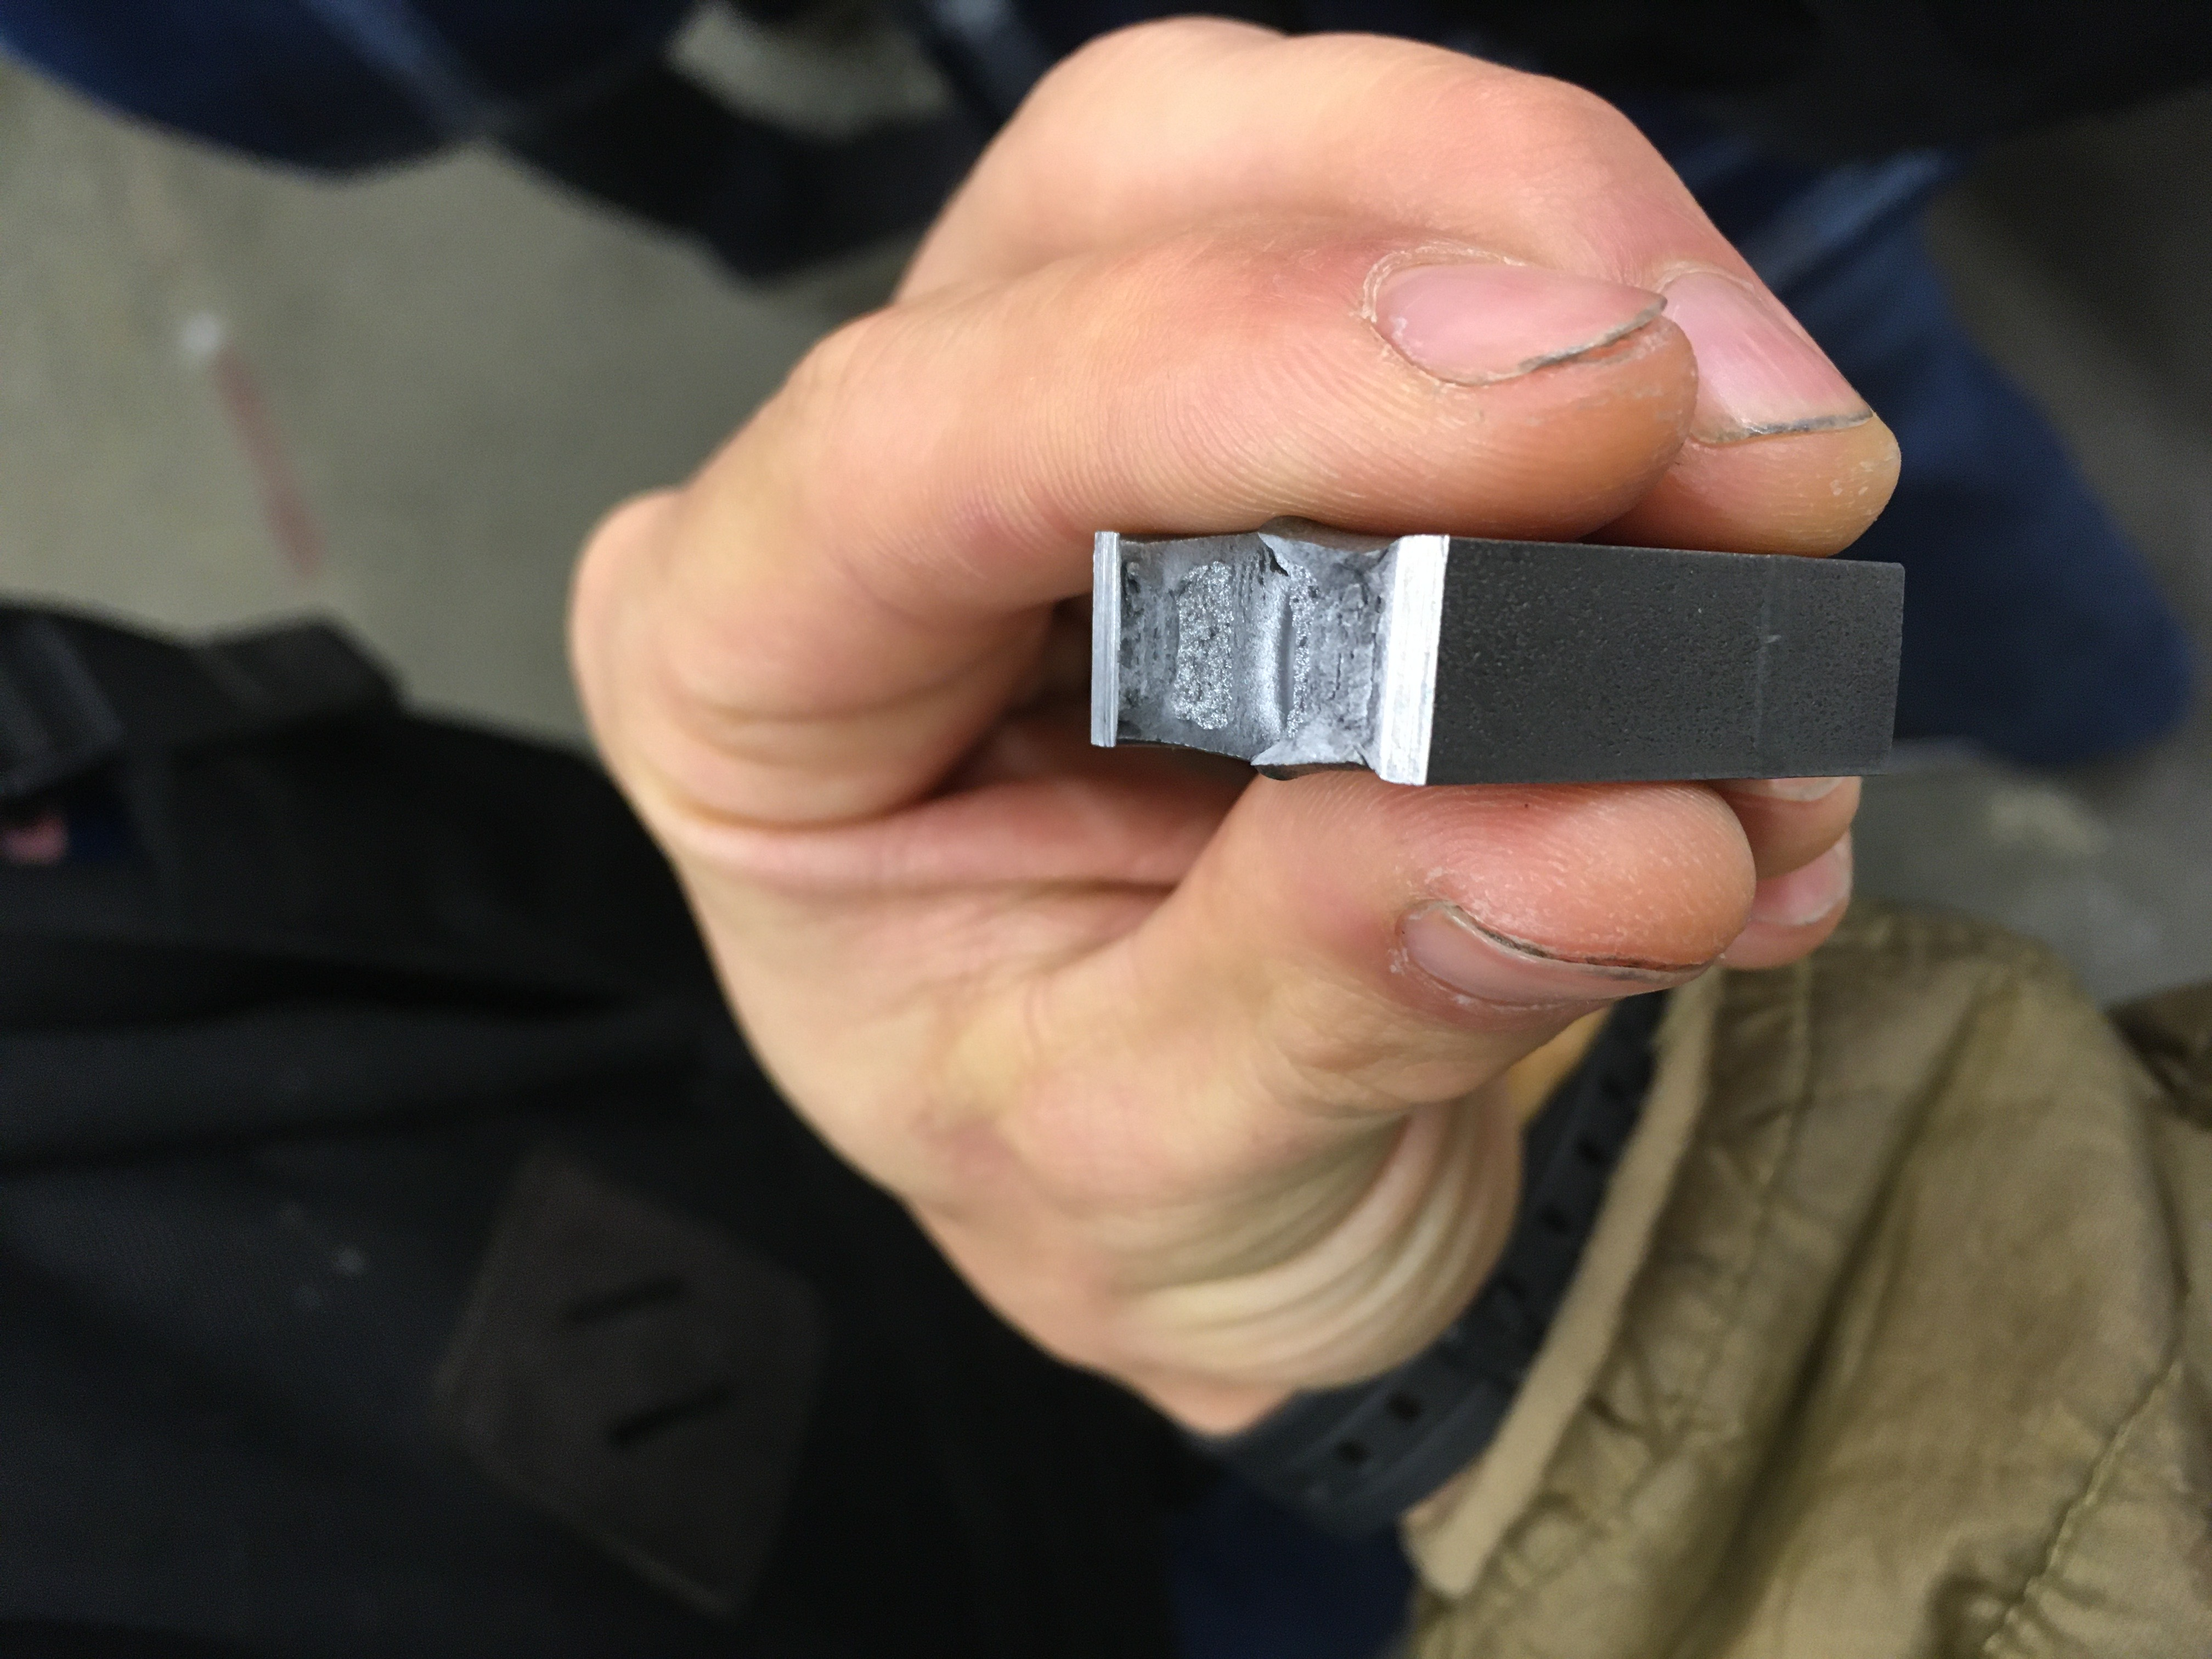
\includegraphics[width=.8\linewidth]{Fe25}
\caption{Steel at \ang{25}C}
\end{subfigure}
\hfill
\begin{subfigure}{.5\textwidth}
\centering
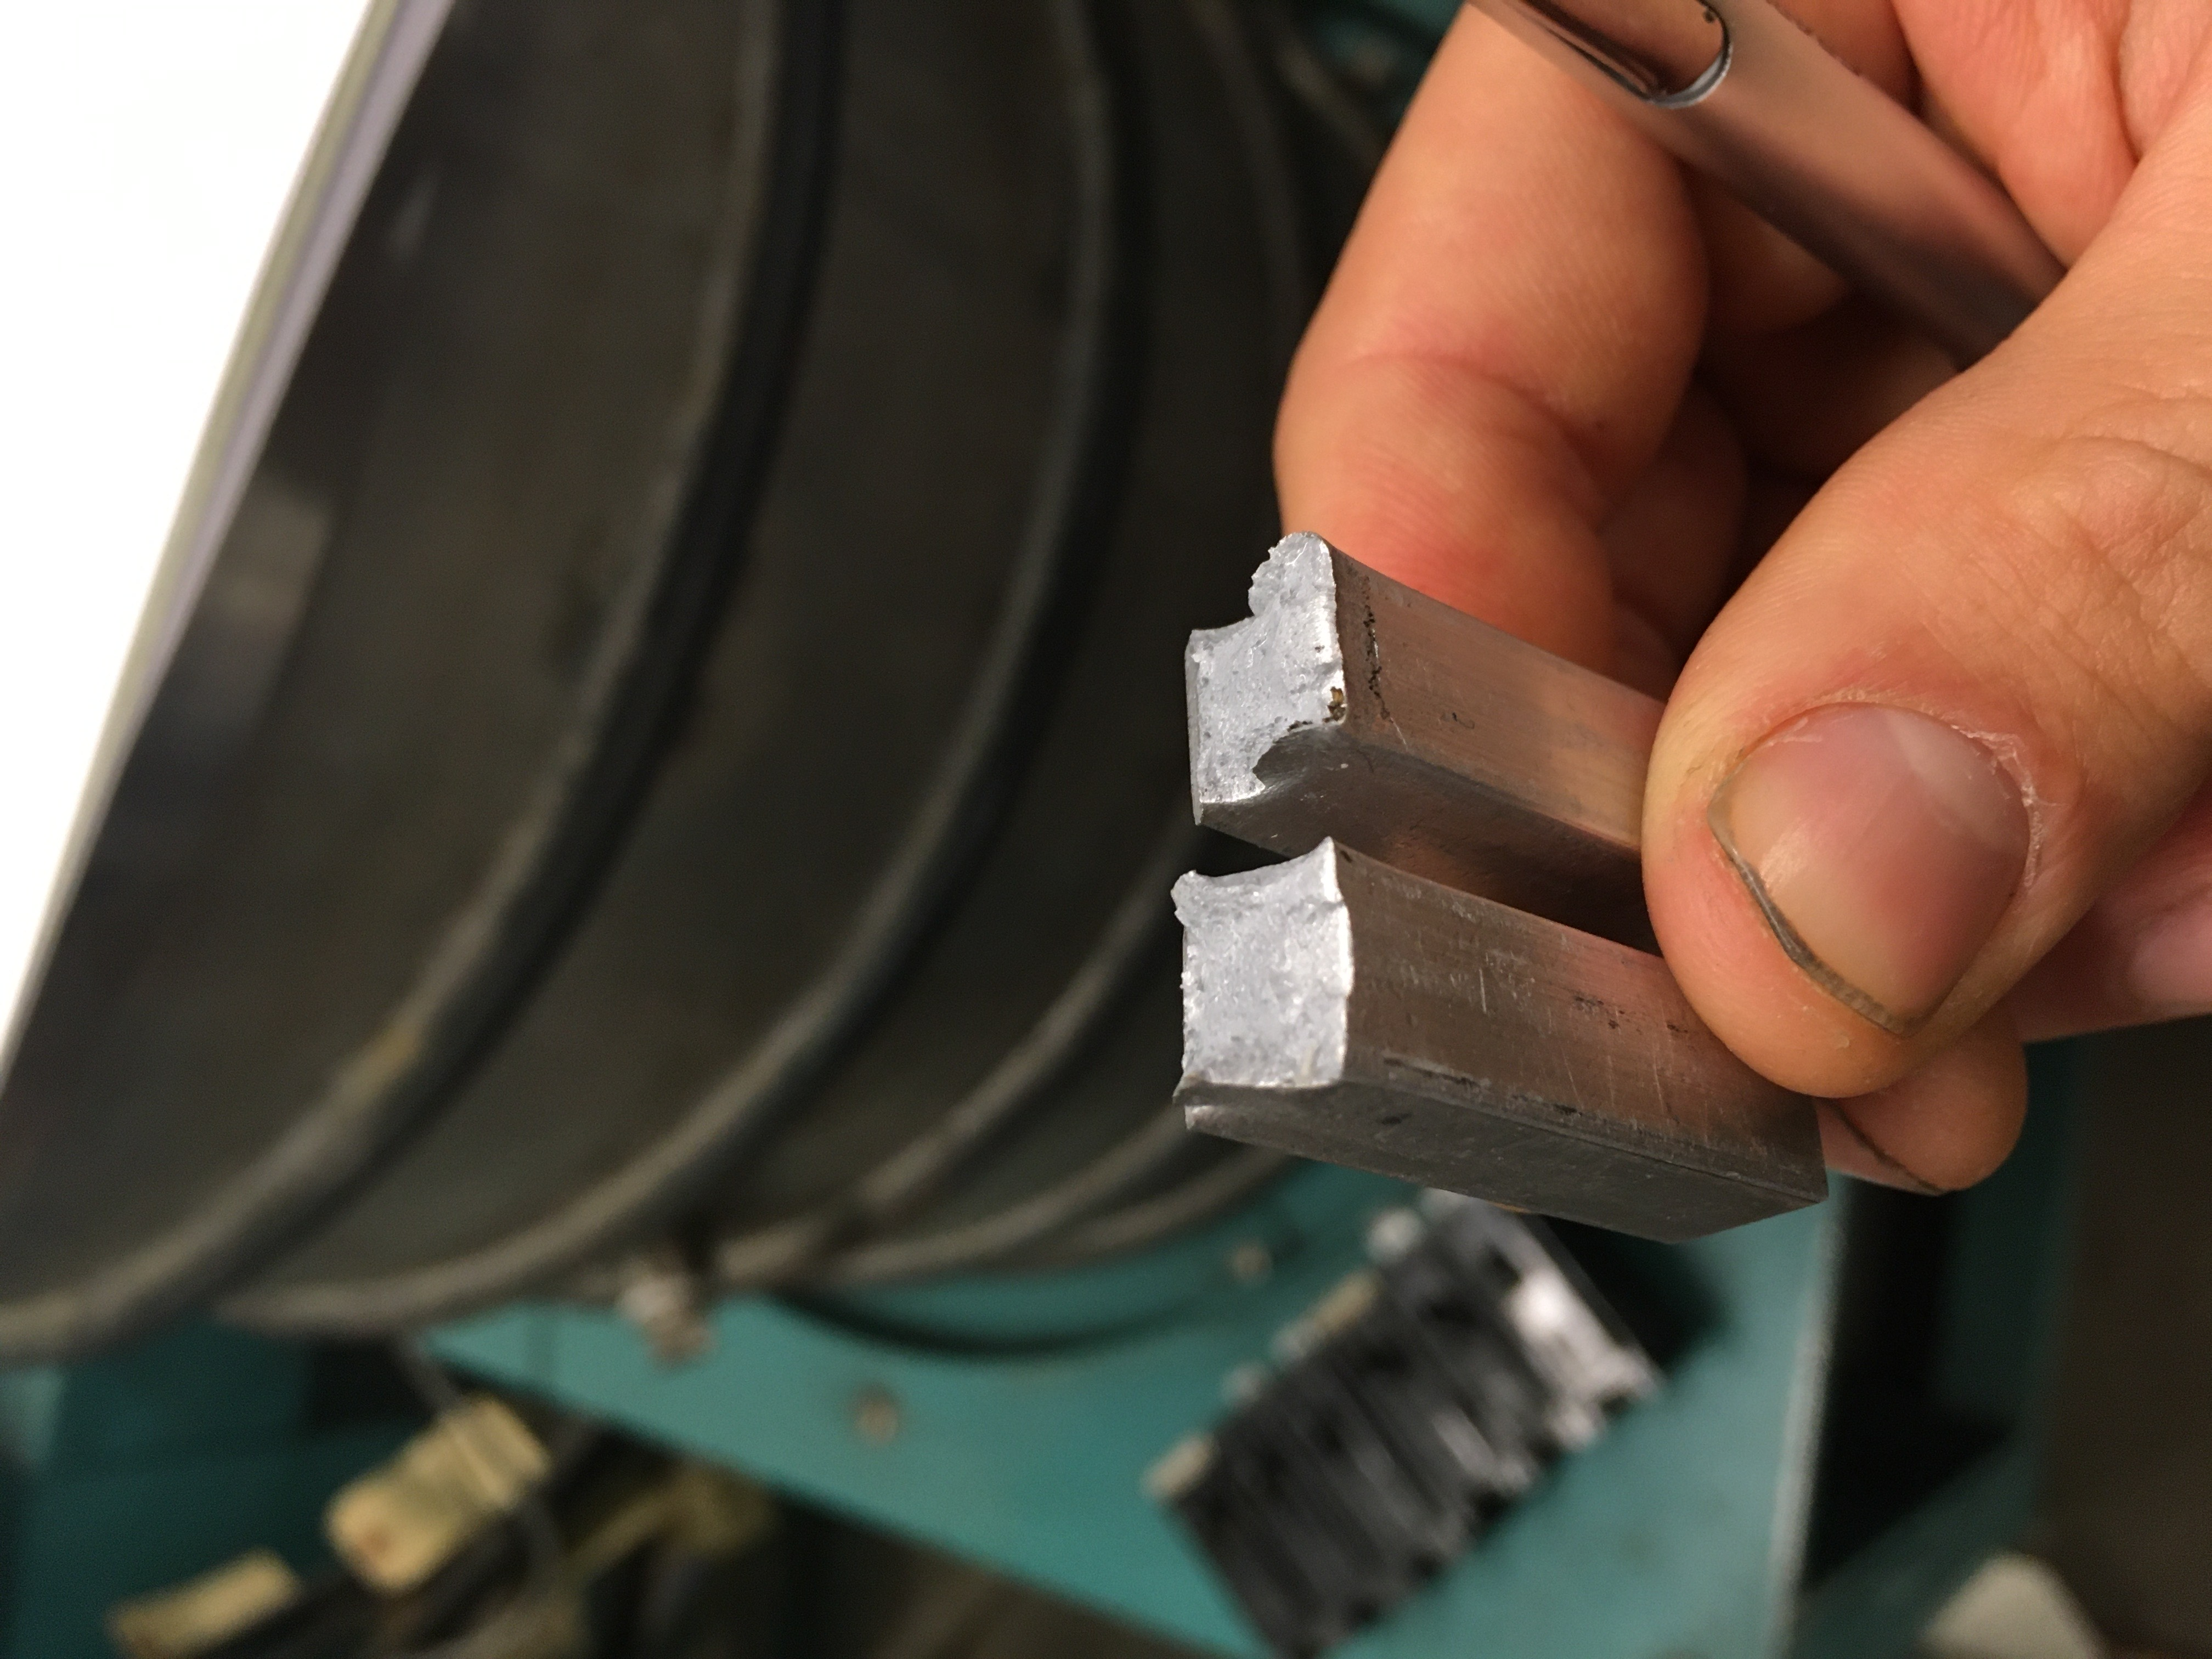
\includegraphics[width=.8\linewidth]{Al-60}
\caption{Aluminum at \ang{-60}C}
\end{subfigure}
\begin{subfigure}{.5\textwidth}
\centering

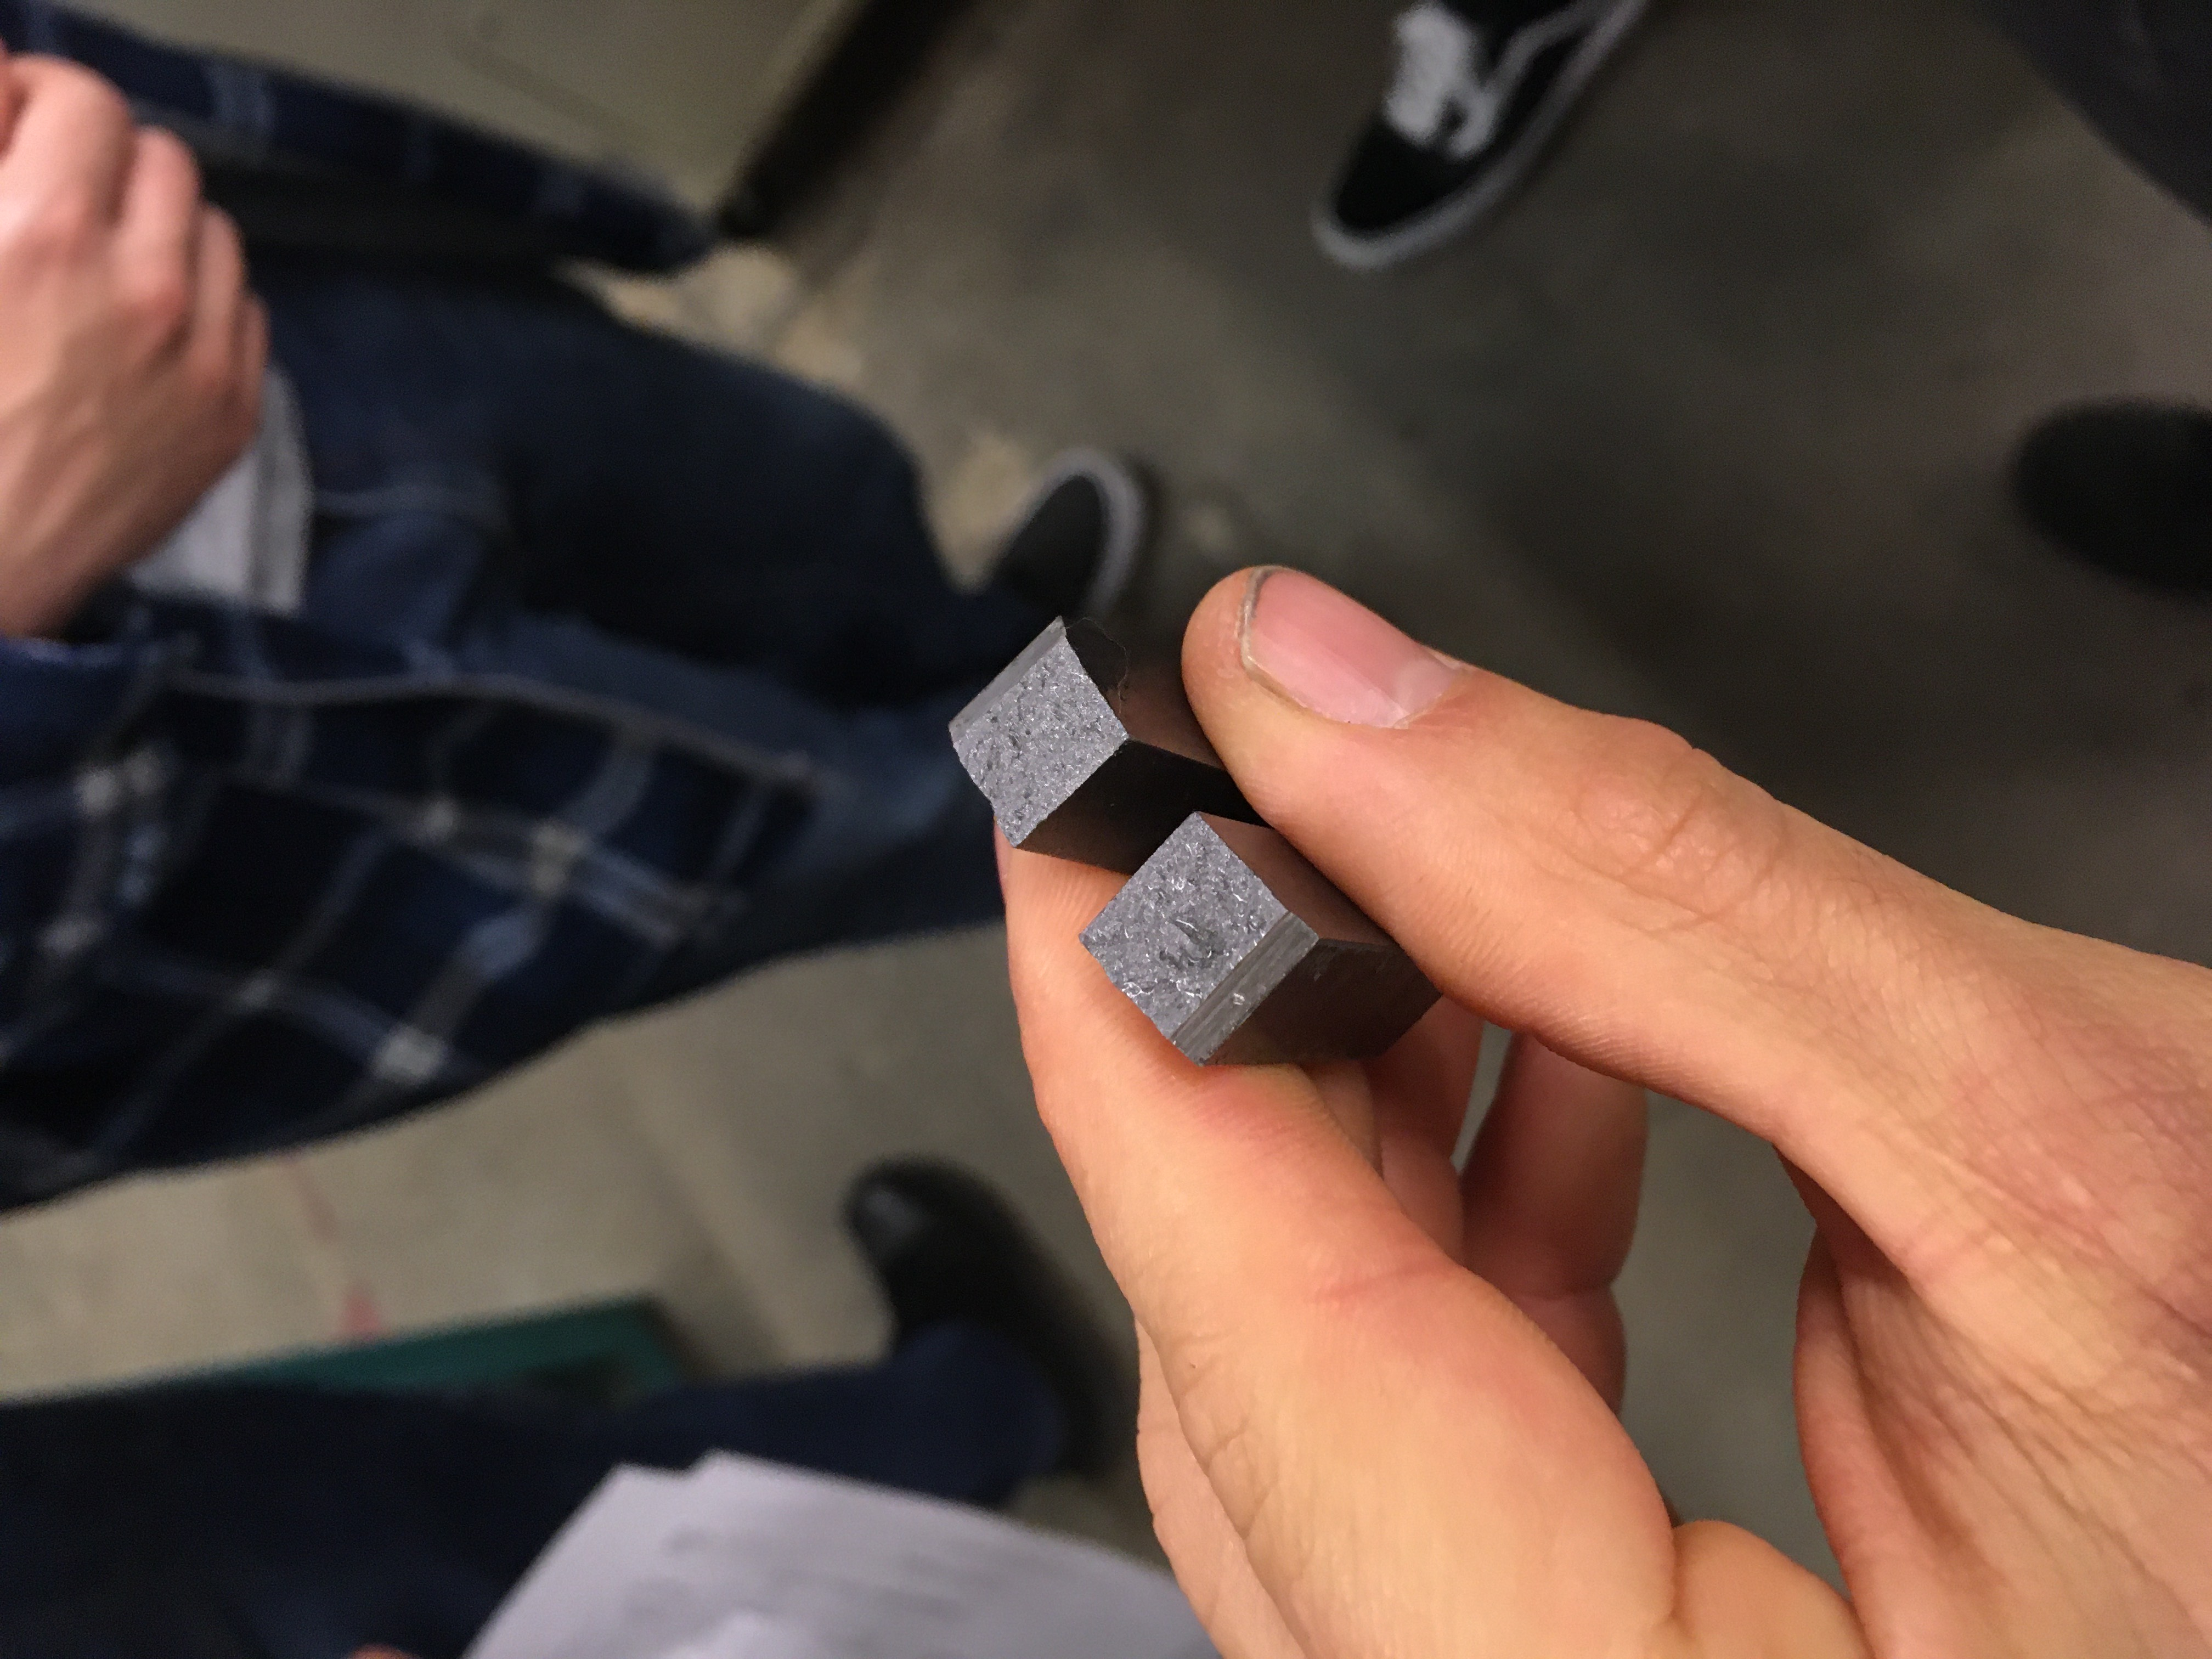
\includegraphics[width=.8\linewidth]{Fe-60}
\caption{Steel at \ang{-60}C}
\end{subfigure}
\end{figure}



\item The steel we tested certainly can not be used to store liquid oxygen which has a boiling point of \ang{-183}C as the material already showed brittle fracture at \ang{-60}C. The aluminum sample did have a decrease in fracture toughness of 23.5\% from 17 ft$\cdot$lbs to 13 ft$\cdot$lbs but aluminum will remain ductile even at very low temperatures due to its FCC crystal structure. Both materials get stronger with decreasing temperature, but the aluminum remains reasonably tough which allows it to be used in cryogenic applications.
\end{enumerate}

\section{Conclusion}
While we only tested our samples at two temperatures, which is insufficient to plot a curve for impact energy versus temperature, but we are still able to tell that the ductile to brittle transition temperature for steel lies somewhere between the temperatures we tested. With more data at more temperatures we would have a more accurate model for the materials we tested. However, even with the few data points we have there is a clear ductile to brittle transition for the steel sample compared to the Aluminum sample (Figure 1). In analyzing the fracture surfaces, we can also see the clear change in fracture surface correlating with a decrease in fracture energy for the steel sample undergoing brittle fracture. For future labs it would be interesting to see how treated steels and steels of various compositions respond to changing temperature, and to see to what temperatures aluminum can be lowered while remaining relatively ductile.

\end{document}